\section{Methods}\label{sec:methods}
%
\subsection{\pyhf{}}\label{subsec:pyhf}

Placeholder for \pyhf{} in methods

%
\subsection{\funcX{}}\label{subsec:funcX}
\funcX{} is a distributed FaaS platform that is designed to support the unique needs of scientific computing. It combines a reliable and easy-to-use cloud-hosted interface with the ability to securely execute functions on distributed endpoints deployed on various computing resources. \funcX{} supports many high performance computing systems and cloud platforms, can use three popular container technologies, and can expose access to heterogeneous and specialized computing resources. The developer interface to funcX is one of its key benefits. Creating a servable function is as easy as writing a python function. Invoking a remote function involves calling a function on an instance of the funcX client class and passing in arguments as required by the remote function.

A funcX endpoint is a logical entity that represents a compute resource. The endpoint is managed by an agent process that allows the funcX service to dispatch functions to that resource for execution. The agent handles authentication and authorization, provisioning of nodes on the compute resource, and monitoring and management. Administrators or users can deploy a funcX agent and register an endpoint for themselves and/or others, providing descriptive (e.g., name, description) metadata. Each endpoint is assigned a unique identifier for subsequent use.

Behind the scenes, funcX uses a heterogeneous executor model based on the Parsl parallel scripting project~\cite{Parsl_paper}.  This architecture uses manager processes which run at a particular compute site. The managers are configured to use one of many different task execution providers such as:
\begin{itemize}
\item HTCondor
\item Slurm
\item Torque
\item Kubernetes
\end{itemize}

With this architecture it is possible to launch tasks on any of these different environments using the same, simple invocation syntax. Resources on different HPCs can be accessed by simply changing the endpoint identifier. The endpoint's configuration has numerous settings to tune the endpoint's use of compute resources to the specific environment and the computational profile of the job at hand. This can be to configure workers to take advantage of small windows of CPU availability, or perhaps allow the workers to wait for a larger allocation to be available. In either event, the funcX service will cause the task to wait and execute as many tasks as it can when the workers are available.  This helps to match the job profiles against a wide variety of compute environments.

%
\subsection{Current and Future FaaS Analysis Facilities}\label{subsec:FaaS_analysis_facilities}

Through the capabilities of \funcX{} and the fitting performance and declarative nature of \pyhf{} there is opportunity to create a fitting FaaS analysis facility blueprint for leveraging the scaling potential at HPC centers and dedicated hardware acceleration resources.
The blueprint can then be replicated in deployment at HPC centers with available resources and allocation.
\Cref{fig:infrastructure_perspective} shows possible cyberinfrastructure and system design prospects, from the viewpoints of developers and uses, to create a deployment of the blueprint.
As a demonstration of the ability to reduce the time to insight such facilities would offer, we use the RIVER HPC system's~\cite{RIVER_HPC} deployment of \funcX{} to simultaneously evaluate the 125 signal hypothesis patches from the published analysis of a search for electroweakinos with the ATLAS detector using the full Run-2 dataset of \(139~\ifb\) of \(\sqrt{s} = 13\,\text{TeV}\) proton-proton collision data~\cite{SUSY-2019-08} with \pyhf{}.
RIVER is able to use \funcX{}'s Slurm task execution provider to leverage the 120 VM cluster for batch jobs.
Each pair of VMs share a hardware node with two Intel Xeon E2650 v3 processors (24 cores), 16 x 16GB TruDDR4 Memory (256GB), two 800GB SATA MLC SSD's (1.6TB), and a 10GigE network --- providing an excellent testing grounds for scaling workflows.

\begin{figure}[!htpb]
    \centering
    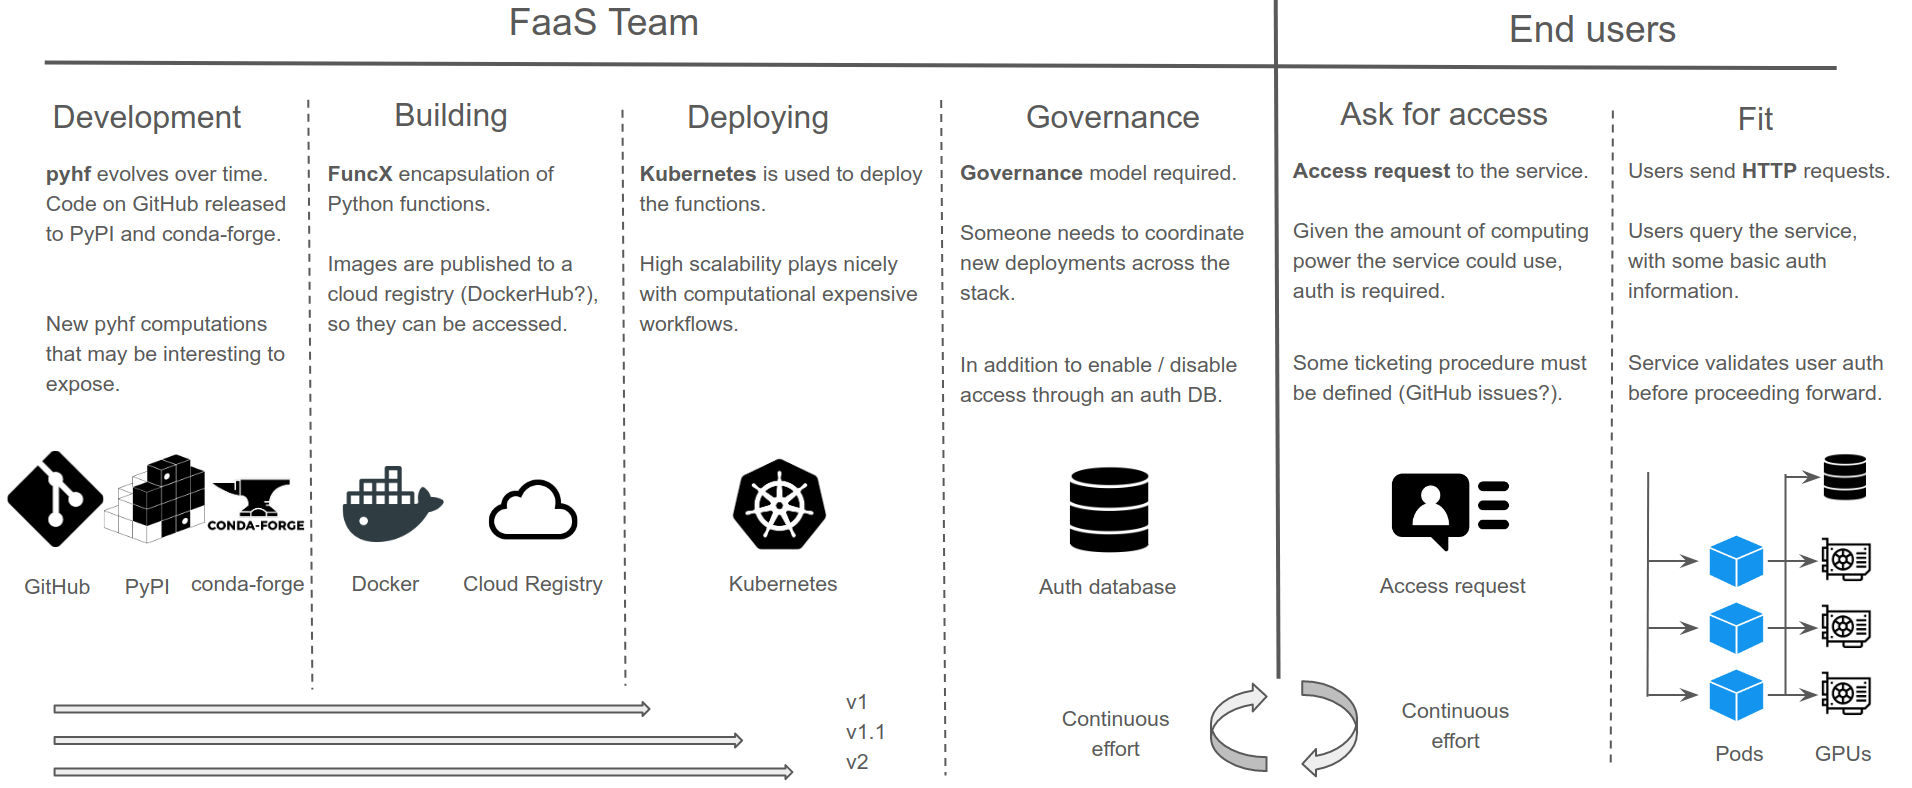
\includegraphics[width=\textwidth]{infrastructure_perspective.png}
    \caption{Example infrastructure design from the developer and user perspectives for a \pyhf{} and \funcX{} based fitting FaaS system for physics analysis.~\cite{portable_inference_workshop}}
    \label{fig:infrastructure_perspective}
\end{figure}
